
\documentclass[11pt,reqno,twocolumn]{article} % use larger type; default would be 10pt

\usepackage{multicol}
\usepackage{my_packages}
\usepackage{tikz_packages}
\usepackage{float}
\tdplotsetmaincoords{60}{125} % view angle in spherical coordinates
\renewcommand{\thesection}{\Roman{section}} 
\renewcommand{\thesubsection}{\thesection.\Roman{subsection}}

\title{Simultaneous landing and mapping on Asteroid Itokawa}
\author{Shankar Kulumani}
% \thanks{PhD Candidate, Department of Mechanical and Aerospace Engineering, Email:~\href{mailto:skulumani@gwu.edu}{skulumani@gwu.edu}}


\date{} % Activate to display a given date or no date (if empty),
         % otherwise the current date is printed 

\begin{document}
\maketitle
\subsubsection*{Motivation}
% Motivation for missions/studying asteroids
Small solar system bodies, such as asteroids and comets, are of significant interest to the scientific community.
These small bodies offer great insight into the early formation of the solar system.
Of particular interest are those near-Earth asteroids (NEA) which inhabit heliocentric orbits in the vicinity of the Earth.
These easily accessible bodies provide attractive targets to support space industrialization, mining operations, and scientific missions.
Furthermore, these asteroids are of keen interest for more practical purposes.
The recent meteor explosions in  2002 over Tagish Lake, Canada or over Chelyabinsk, Russia in 2013 are clear evidence of the risk of asteroid impacts on the Earth.
These asteroids, which released an energy equivalent to \SI{5}{\kilo\tonne} of TNT, are estimated to strike the Earth on average every year~\cite{brown2002}.
Larger bodies, such as the \SI{60}{\meter} object that exploded over Tunguska, Russia in 1908, release the energy equivalent to \SI{10}{\mega\tonne} of TNT and will occur on average every \num{1000} years.
In spite of the significant interest in asteroid deflection, and the extensive research by the community, the operation of spacecraft in their vicinity remains a challenging problem.

\subsubsection*{Research Question}
% describe our approach in this paper
In this work, we develop a orbit and landing scheme for spacecraft on an asteroid.
The main objective is to construct the coupled equations of motion of a rigid spacecraft about an asteroid.
This accurate dynamic model is then used to derive a nonlinear controller for the tracking of a landing trajectory.
In contrast to much of the previous work, we explicitly consider the gravitational coupling between the orbit and attitude dynamics.
In addition, we utilize a polyhedron potential model to represent the shape of the asteroid, which results in an exact closed form expression of the gravitational potential field~\cite{werner1994,werner1996}.

In order to determine the shape of the asteroid, we model a laser ranging sensor (LIDAR) on a maneuvering spacecraft.
The LIDAR is able to provide depth measurements of the surface of the asteroid.
Given a set of depth measurements it is possible to compute the shape, and hence gravitational potential of the asteroid.
Computing the shape of the asteroid on a continual basis avoids the long delay and computational complexity of current asteroid operations.
Furthermore, the updated gravitional model enables a spacecraft to autonomously transition from a mapping orbit, directly to landing.

\subsection*{Mathematical Formulation}\label{se:mathematical_problem}
The gravitational potential around a constant density asteroid can be defined entirely from its shape.
We model the asteroid shape as a set of vertices and triangular faces.
Given this shape the potential at any point around the asteroid is defined as
\begin{align}\label{eq:potential}
    U(\vecbf{r}) &= \frac{1}{2} G \sigma \sum_{e \in \text{edges}} \vecbf{r}_e \cdot \vecbf{E}_e \cdot \vecbf{r}_e \cdot L_e \nonumber\\
                 &- \frac{1}{2}G \sigma \sum_{f \in \text{faces}} \vecbf{r}_f \cdot \vecbf{F}_f \cdot \vecbf{r}_f \cdot \omega_f \in \R^1,
\end{align}
In this work, we consider the motion of a dumbbell model of a spacecraft about an asteroid.
The dumbbell spacecraft consists of two masses connected by a massless rod and is a well-known representation of a multi body spacecraft.
Furthermore, the dumbbell model captures the important interactions of the coupling between orbital and attitude dynamics. 

\subsection*{Technical Approach}

\begin{figure}
    \centering
    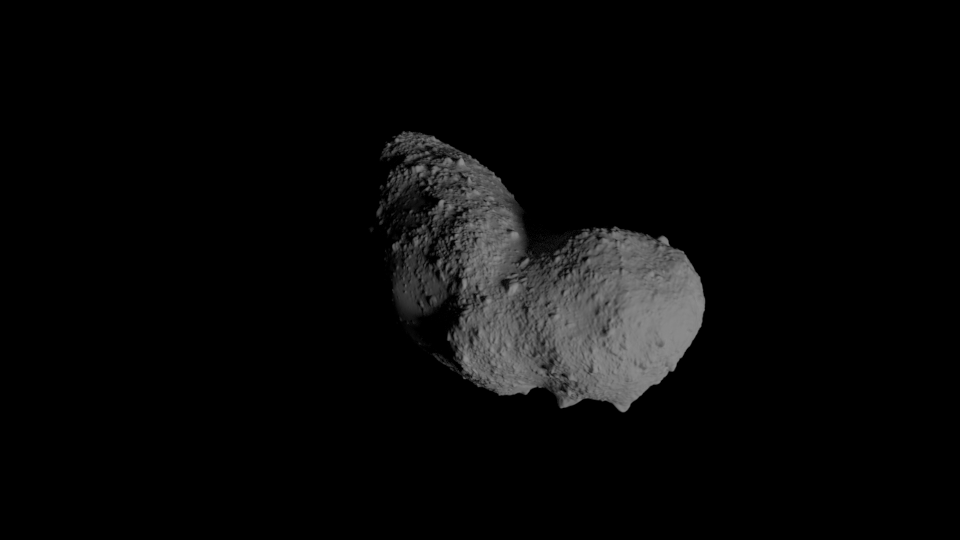
\includegraphics[width=\columnwidth,trim={50mm 30mm 50mm 30mm},clip]{figures/itokawa_blender.png}
    \caption{Realistic rendering of Itokawa}
\end{figure}

Prior to the arrival at the asteroid, it is only possible to determine a coarse ellipsoidal approximation of the shape of an asteroid from ground based measurements. 
As a result, the dynamic model of the gravitational environment will be inaccurate until the shape of the asteoriod is determined. 
We simulate measurements of the surface using a laser range finder mounted on the spacecraft.
A laser depth sensor, or LIDAR, provides the distance to the surface by measuring the round trip time of flight of reflections from the surface.
We simulate the measurements of the surface using an efficient ray casting technique based on a modified binary space partition tree~\cite{formella1995}.
\begin{figure}[htbp]
    \centering
    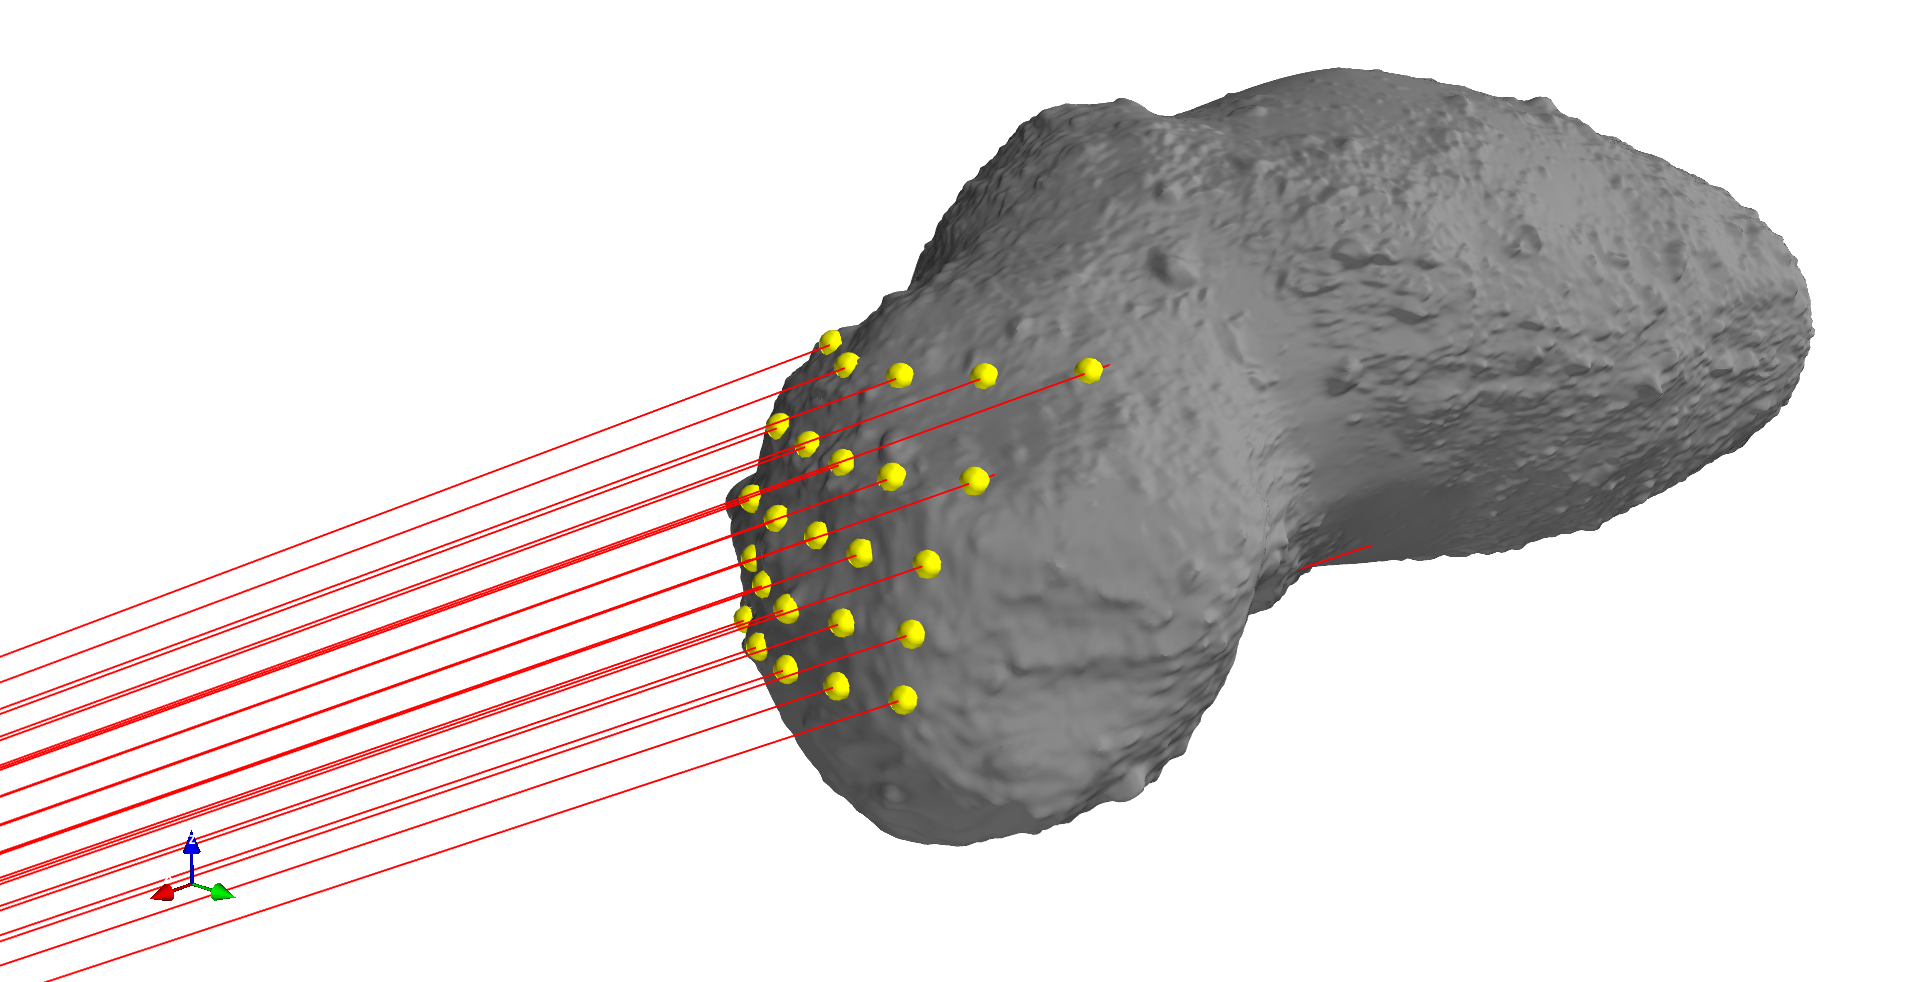
\includegraphics[width=\columnwidth]{figures/raycasting.png}
    \caption{Ray Casting example around Itokawa\label{fig:raycasting}}
\end{figure}
\Cref{fig:raycasting} shows an example of ray casting to determine depth measurements of the surface of asteroid Itokawa.
The rays from the spacecraft to the asteroid are shown in red, while the measurements of the surface are shown in yellow.
By combining many measurements of the surface a  point cloud representation of the asteroid is generated.

The shape of the asteroid is computed in near real time instead of requiring ground based computation.
This allows for a much larger class of missions and removes the need for the spacecraft to remain in a mapping specific orbit for long periods of time.
Instead, the spacecraft is able to autonomously compute the shape while maneuvering.
The final step is to reconstruct the shape of the asteroid from the depth measurements~\cite{hoppe1992}.
\subsubsection*{Contribution}
We will simultaneously derive the shape of the asteroid while maneuvering.
This alleviates the long and labor intensive efforts to determine the shape in a specific mapping orbit.
Instead, our approach allows for online shape generation and enables for responsive and short duration missions to the asteroid surface.
\bibliographystyle{plain}
\bibliography{library.bib}

\end{document}
